
\chapter{Linear Algebra Applications}

This chapter covers the following ideas.  

\begin{enumerate}

\item Find the currents in electrical systems involving batteries and resistors, using both Gaussian elimination and Cramer's rule.
\item Find interpolating polynomials. Use the transpose and inverse of a matrix to solve the least squares regression problem of fitting a line to a set of data.
\item Find the partial fraction decomposition of a rational function. Utilize this decomposition to integrate rational functions.
\item Describe a Markov process. Explain how an eigenvector of the eigenvalue $\lambda=1$ is related to the limit of powers of the transition matrix.
\item Explain how to generalize the derivative to a matrix. Use this generalization to locate optimal values of the function using the second derivative test. Explain the role  of eigenvalues and eigenvectors in the second derivative test.
\end{enumerate}


\section{Kirchoff's Electrial Laws}
Gustav Kirchoff discovered two laws of electricity that pertain to the conservation of charge and energy.  To describe these laws, we must first discuss voltage, resistance, and current.  Current is the flow of electricity, and often it can be compared to the flow of water.  As a current passes across a conductor, it encounters resistance. Ohm's law states that the product of the resistance $R$ and current $I$ across a conductor equals the voltage $V$, i.e. $RI=V$. If the voltage remains constant, then a large resistance corresponds to a small current. A resistor is an object with high resistance which is placed in an electrical system to slow down the flow (current) of electricity.  Resistors are measured in terms of ohms, and the larger the ohms, the smaller the current.  Figure \ref{ecir} illustrates two introductory electrical systems. 



\begin{figure}[htb]
\begin{center}
\begin{tabular}{cc}
\input{03-Linear-Algebra-Applications/electric-circuit-2-loops}
&
\input{03-Linear-Algebra-Applications/electric-circuit-3-loops}
\\
Two Loop System & Three Loop System
\end{tabular}\end{center}
\caption{Electrical Circuit Diagrams.}
\label{ecir}\end{figure}
In this diagram, wires meet at nodes (illustrated with a dot).  
Batteries and voltage sources (represented by 
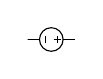
\begin{tikzpicture}[scale=.15,rotate=-90]
%	\useasboundingbox (-.5,-3) rectangle (.5,3);
	\clip (-1,-2) rectangle (1,2);
	\draw (0,0) circle (1cm);
	\draw (.3,.5) -- (-.3,.5);
	\draw (0,.2) -- (0,.8);
	\draw (.3,-.5) -- (-.3,-.5);
	\draw (0,1) -- (0,3);
	\draw (0,-1) -- (0,-3);
\end{tikzpicture}
or other symbols)
supply a voltage of $E$ volts.  At each node the current may change, so the arrows and letters $i$ represent the different currents in the electrical system. The electrical current on each wire may or may not follow the arrows drawn (a negative current means that the current flows opposite the arrow). Resistors are depicted with the symbol 	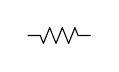
\begin{tikzpicture}[scale=.2,rotate=90]
%	\useasboundingbox (0,-3) rectangle (0,3);
	\clip (-.5,-2) rectangle (.5,2);
	\draw (0,-3) -- ++(0,1.8) -- ++(.5,.2) 
		-- ++(-1,.4) -- ++(1,.4)
		-- ++(-1,.4) -- ++(1,.4)
		-- ++(-1,.4) -- ++(.5,.2)
		-- ++(0,1.8) ;
	\end{tikzpicture}
, and the letter $R$ represents the ohms. 

Kirchoff discovered two laws. They both help us find current in a system, provided we know the voltage of any batteries, and the resistance of any resistors. 
\begin{enumerate}
	\item Kirchoff's current law states that at every node, the current flowing in equals the current flowing out (at nodes, current in = current out). 
	\item Kirchoff's voltage law states that on any loop in the system, the directed sum of voltages supplied equals the directed sum of voltage drops (in loops, voltage in = voltage out). 
\end{enumerate}

Let's use Kirchoff's laws to generate a system of equations for the two loop system. 
\begin{enumerate}
	\item First we will examine Kirchoff's current law. At the first node (top middle), current $i_1$ flows in while $i_2$ and $i_3$ flow out. Kirchoff's current law states that $i_1=i_2+i_3$ or $i_1-i_2-i_3=0$.  At the second node, both $i_2$ and $i_3$ are flowing in while $i_1$ flows out. This means that $i_2+i_3=i_1$ or $-i_1+i_2+i_3=0$. This second equation is the same as multiplying both sides of the first by $-1$ (so we say the 2nd equation depends on the first). 
	\item We now look at Kirchoff's voltage law. Pick a loop and work your way around the loop in a clockwise fashion. Each time you encounter a battery or resistor, include a term for the voltage supplied $E$ on the left side of an equation, and the voltage drop (resistance times current $Ri$) on the right. If you encounter a battery or resistor as you work against the current, then times that term by $-1$. The left loop has a battery with voltage $E$ and the resistor contributes a drop in voltage of $R_1 i_2$ volts.  An equation for the first loop is $E=R_1i_1+R_2i_2$. On the right loop we encounter along current $i_3$ a resistor with resistance $R_3$ ohms.  While working our way against the arrow drawn on $i_2$, we encounter an $R_2$ ohm resistor.  There are no batteries on the second loop. The two resistors give us the equation $0=-R_2 i_2 +R_3i_3$. 
\end{enumerate}
We can now write a system of equations involving the unknowns $i_1,i_2,i_3$, put it in matrix form, and then solve
$$
\begin{array}{rl}
i_1-i_2-i_3&=0\\
-i_1+i_2+i_3&=0\\
R_1i_1+R_2i_2&=E\\
-R_2 i_2 +R_3i_3&=0
\end{array}
\xrightarrow{\text{matrix form}}
\begin{bmatrix}[ccc|c]
1&-1&-1&0\\
-1&1&1&0\\
R_1&R_2&0&12\\
0&-R_2&R_3&0
\end{bmatrix}
$$$$
\xrightarrow{\text{rref}}
\begin{bmatrix}[ccc|c]
 1 & 0 & 0 & \dfrac{E R_2+ E R_3}{R_1 R_2+R_1 R_3+R_2R_3} \\
 0 & 1 & 0 & \dfrac{E R_3}{R_1 R_2+R_1 R_3+R_2R_3} \\
 0 & 0 & 1 & \dfrac{E R_2}{R_1 R_2+R_1 R_3+R_2R_3} \\
 0 & 0 & 0 & 0
\end{bmatrix}.
$$
The reason we have a row of zeros at the bottom of or system is because the two rows corresponding to the nodes are linearly dependent.  Hence, when we reduce the matrix that dependence relation becomes a row of zeros.

A similar computation can be done for the three loop system. There are 6 unknown currents, 4 nodes, and 3 loops.  This will give us 7 equations with 6 unknowns.  The 4 equations from the nodes will again contribute rows which are linearly dependent, which means you can always ignore an equation from one of the nodes. Reduction will give a unique solution. In the homework, you are asked to setup systems of equations for various electrical systems, and then solve them. 


\begin{example} \label{electrical example}Let's look at an example which involves numbers.  Suppose $E=12$ (a 12 volt battery) and the resistors have $R_1=2, R_2=R_3=4$ ohms. The top node gives the equation $i_1=i_2+i_3$ (remember flow in equals flow out). We'll skip the bottom node.  The left loop gives the equation $12 = 2i_1+4i_2$, while the right loop gives the equation $0=-4r_2+4r_3$.  We now 
$$
\begin{array}{rl}
i_1-i_2-i_3&=0\\
2i_1+4i_2&=12\\
-4 i_2 +4i_3&=0
\end{array}
\xrightarrow{\text{matrix form}}
\begin{bmatrix}[ccc|c]
1&-1&-1&0\\
2&4&0&E\\
0&-4&4&0
\end{bmatrix}
\xrightarrow{\text{rref}}
\begin{bmatrix}[ccc|c]
 1 & 0 & 0 & 3\\
 0 & 1 & 0 & 3/2\\
 0 & 0 & 1 & 3/2
\end{bmatrix}
$$
which tells us the currents are $i_1=3$, $i_2=3/2$, and $i_3=3/2$.
\end{example}






\subsection{Cramer's Rule}
Cramer's rule is a theoretical tool which gives the solution to any linear system $A\vec x = \vec b$ with $n$ equations and $n$ unknowns, provided that there is a unique solution.  Let $D=\det(A)$. Let $D_i$ be the determinant of the matrx formed by replacing the $i$th column of $A$ with $\vec b$.  Then Cramer's rule states that $x_1 = \frac{D_1}{D},x_2 = \frac{D_2}{D},\ldots, x_n = \frac{D_n}{D}$. We may prove it in class with pictures which connect determinants to area (eventually I'll add this to an appendix)\note{appendix problem}. This method of solving a system of equations is quickly doable for 2 by 2 and 3 by 3 systems, but becomes computationally inefficient beyond (as computing determinants is time consuming and numerically unstable on large matrices). For large systems, it is better to use Gaussian elimination.  Cramer's rule is a powerful theoretical tool, and can simplify generic computations. 

\begin{example}
Let's solve $
\begin {bmatrix} 1&2&0\\-2&0&1\\0&3&-2\end {bmatrix} 
\begin {bmatrix} x_1\\x_2\\x_3\end {bmatrix} 
=  \begin{bmatrix} 2\\-2\\1\end {bmatrix}
$ using Cramer's rule.  
We compute the determinant of the coefficient matrix first to obtain
$$D=\begin{vmatrix} 1&2&0\\-2&0&1\\0&3&-2\end {vmatrix} = -11.$$ Next we replace each column of the coefficient matrix with the right column of our augmented system and compute the three determinants to obtain
$$
\begin{vmatrix} 2&2&0\\-2&0&1 \\1&3&-2\end {vmatrix}   =-12,
\begin{vmatrix} 1&2&0\\-2&-2&1 \\0&1&-2\end {vmatrix} =-5, 
\begin{vmatrix} 1&2&2\\-2&0&-2 \\0&3&1\end {vmatrix} =-2 .$$
Cramer's rule requires that we divide each of these determinants by the original determinant, giving the solution $x_1=12/11, x_2 = 5/11, x_3 = 2/11$.  Using Gaussian Elimination, we obtain the same solution 
$$ \begin {bmatrix}[ccc|c] 1&2&0&2\\-2&0&1&-2\\0&3&-2&1\end {bmatrix}\xrightarrow{\text{rref}}
\begin {bmatrix}[cccc] 1&0&0&12/11
\\0&1&0&5/11\\0&0&1&2/11\end {bmatrix} 
, $$
however the arithmetic involved in keeping track of fractions or really large integers becomes much more difficult by hand without Cramer's rule.
\end{example}

\begin{example}
Consider the electrical system in Example \ref{electrical example} where $E=12$, $R_1=2$, and $R_2=R_3=4$. The corresponding augmented matrix we used to solve this system was 
$$
\begin{bmatrix}[ccc|c]
1&-1&-1&0\\
2&4&0&E\\
0&-4&4&0
\end{bmatrix}, 
A=
\begin{bmatrix}1&-1&-1\\2&4&0\\0&-4&4\end{bmatrix}, 
b=\begin{bmatrix}
0\\
E\\
0
\end{bmatrix},D=\begin{vmatrix} 1&-1&-1\\2&4&0\\0&-4&4 \end {vmatrix} =32. 
$$ 
We now replace each column with $\vec b$ and compute the determinant of the corresponding matrix (remember to cofactor along the column which contains $0,12,0$ to do this quickly)
$$ 
D_1=\begin{vmatrix} 0&-1&-1\\12&4&0\\0&-4&4 \end {vmatrix} =96,
D_2=\begin{vmatrix} 1&0&-1\\2&12&0\\0&0&4 \end {vmatrix} =48, 
D_3=\begin{vmatrix} 1&-1&0\\2&4&12\\0&-4&0 \end {vmatrix} =48. 
$$
Dividing each of these by the determinant of the original matrix gives the solution $i_1 = 96/32 = 3$, $i_2=i_3=48/32 = 3/2$, which matches the solution we found using row reduction in the previous section. 
\end{example}



















\section{Find Best Fit Curves}
\subsection{Interpolating Polynomials}
Through any two points (with different $x$ values) there is a unique line of the form $y=mx+b$. If you know two points, then you can use them to find the values $m$ and $b$.  Through any 3 points (with different $x$ values) there is a unique parabola of the form $y=ax^2+bx+c$, and you can use the 3 points to find the values $a,b,c$.  As you increase the number of points, there is still a unique polynomial (called an interpolating polynomial) with degree one less than the number of points, and you can use the points to find the coefficients of the polynomial. In this section we will illustrate how to find interpolating polynomials, and show how the solution requires solving a linear system. Cramer's rule or Gaussian elimination will give us the solution. 

To organize our work, let's first standardize the notation.  Rather than writing $y=mx+b$, let's write $y=a_0+a_1 x$ (where $a_0=b$ and $a_1=m$). For a parabola, let's write $\ds y=a_0 + a_1 x+ a_2 x^2 = \sum_{k=0}^{2} a_k x^k$. We can now write any polynomial in the form $$\ds y = a_0 + a_1 x+ \cdots + a_n x^n = \sum_{k=0}^n a_k x^k.$$ By standardizing the coefficients, we can use summation notation to express any degree polynomial by changing the $n$ on the top of the summation sign. Now that our notation is organized, let's use it to find a polynomial through 3 points.

\begin{example}
Let's find a parabola through the three points $(0, 1), (2, 3), (4, 7)$.  The polynomial is $y=a_0 +a_1 x+a_2 x^2$ and our job is to find the three constants $a_0, a_1, a_2$.  Since we have three points, we put these points into the equation to obtain the three equations
$$
a_{{0}}=1 \quad \quad 
a_{{0}}+2\,a_{{1}}+4\,a_{{2}}=3 \quad \quad 
a_{{0}}+4\,a_{{1}}+16\,a_{{2}}=7
$$
This is a linear system with 3 equations and 3 unknowns.  We now write the system in matrix form and reduce it
$$
\begin{bmatrix}[ccc|c] 
1&0&0&1\\
1&2&4&3\\
1&4&16&7
\end {bmatrix}
\xrightarrow{\text{rref}}
\begin{bmatrix}[ccc|c]
1&0&0&1\\
0&1&0&1/2\\
0&0&1&1/4
\end {bmatrix} 
.$$
The reduce row echelon form tells us that the coefficients are $a_0 = 1, a_1= 1/2, a_2=1/4$, which means our parabola is $y=1+\frac12 x+ \frac 14 x^2$. Cramer's rule gives $D=16, D_1=16, D_2=8, D_3=4$, and so $a_0 = 16/16=1, a_1=8/16=1/2, a_2=4/16=1/4$, the same as with Gaussian elimination. 

Once you have obtained your interpolating polynomial, you can always check your work by putting the points back into your new equation. When $x=0$ we have $y=1+0+0=1$, when $x=2$ we have $1+1+1=3$, and when $x=4$ we have $1+2+4=7$, which means the parabola passes through the three points (0,1), (2,3), and (4,7) as needed.  
\end{example}

In the example above, notice that powers of $x$ appear as the coefficients of our coefficient matrix, and we augment that matrix by the $y$ values. This is the general pattern for finding an interpolating polynomial. The diagram below shows the general method for finding an interpolating polynomial through three points.
\begin{center}
\begin{tabular}{c}
$(x_1,y_1),(x_2,y_2),(x_3,y_3)$ \\
 $
\begin{bmatrix}[ccc|c] 
x_1^0=1&x_1^1&x_1^2&y_1\\
1&x_2^1&x_2^2&y_2\\
1&x_3^1&x_3^2&y_3
\end {bmatrix}
\xrightarrow{\text{rref}}
\begin{bmatrix}[ccc|c]
1&0&0&a_0\\
0&1&0&a_1\\
0&0&1&a_2
\end {bmatrix} 
$
\\
 $y=a_0+a_1x+a_2x^2$
\end{tabular}
\end{center}
Finding an interpolating polynomial through 4 points is very similar, you just have to add one more row and column to the matrix and repeat the process.
\begin{center}
\begin{tabular}{c}
$(x_1,y_1),(x_2,y_2),(x_3,y_3),(x_4,y_4)$\\
$
\begin{bmatrix}[cccc|c] 
1&x_1^1&x_1^2&x_1^3&y_1\\
1&x_2^1&x_2^2&x_2^3&y_2\\
1&x_3^1&x_3^2&x_3^3&y_3\\
1&x_4^1&x_4^2&x_4^3&y_4
\end {bmatrix}
\xrightarrow{\text{rref}}
\begin{bmatrix}[cccc|c]
1&0&0&0&a_0\\
0&1&0&0&a_1\\
0&0&1&0&a_2\\
0&0&0&1&a_3
\end {bmatrix} 
$\\
$y=a_0+a_1x+a_2x^2+a_3x^3$
\end{tabular}
This pattern generalizes to all dimensions. Remember that the $x$ values must be different (a function requires only one output for each input). Once you have obtained your solution, remember that you can easily check if your solution is correct by plugging the points into your equation. 
\end{center}





















\subsection{Least Squares Regression}
Interpolating polynomials give a polynomial which passes through every point listed. While they pass through every point in a set of data, the more points the polynomial must pass through, the more the polynomial may have to make large oscillations in order to pass through each point.  Sometimes a simple line or parabola is desired that passes near the points and gives a good approximation of a trend in the data. When I needed to purchase a minivan for my expanding family, I gathered mileage and price data for about 40 cars from the internet. I plotted this data and discovered an almost linear downward trend (as mileage increased, the price dropped).  Using this data I was able to create a line to predict the price of a car.  I then used this data to talk the dealer into dropping the price of their car by over \$1000. \note{I need to find this data on our computer and put a graph here} Finding an equation of this line, called the least squares regression line, is the content of this section. In other words, if you have 3 or more points, how do you find a line that is "closest" to passing through these points?  The least squares regression line is used to find trends in many branches of science, in addition to haggling for lower prices when buying a car. Statistics builds upon this idea to provide powerful tools for predicting the future.

Let's introduce the idea with an example. Let's find a line that is closest to passing through the three points $(0,1)$, $(2,3)$, and $(4,6)$.  Since the points are not collinear, there is not a line through all three.  Suppose for a moment that there were a line of the form $y=b+mx=a_0+a_1x$ that did pass through the points. Plug our 3 points into the equation $b+mx=y$, which gives the system of equations 
$$\begin{cases}b=1\\b+2m=3\\b+4m=6\end{cases}
\xrightarrow{\text{augmented matrix}}
\begin{bmatrix}[cc|c]1&0&1\\1&2&3\\1&4&6\end{bmatrix}
\xrightarrow{\text{matrix eqn}}
\begin{bmatrix}1&0\\1&2\\1&4\end{bmatrix}
\begin{bmatrix}b\\m\end{bmatrix}
=\begin{bmatrix}3\\1\\6\end{bmatrix}.
$$
Notice that the system can be written in matrix form $A\vec x = \vec b$ where $A$ contains a column of 1's and $x$ values, and $\vec b$ is a column of $y$ values. If you try to reduce this matrix, you will discover the system is inconsistent (has no solution) which should not be a surprise since there is no line which passes through these three points. Notice that there are more equations (3 equations) than variables ($b$ and $m$), which means the system is over determined. 

While there is no solution, can we still use our matrix equation to find a solution? Is there a way to reduce the number of rows in our system, so that the resulting system has only 2 rows? If we multiply on the left by a 2 by 3 matrix, we would obtain a system with 2 rows instead of 3, and the rows of the new matrix would be linear combinations of the rows of our original matrix.  The only 2 by 3 matrix in this problem is the transpose of A.  So let's multiply both sides of the matrix equation by the transpose of A, and see what happens:
$$A = \begin{bmatrix}1&0\\1&2\\1&4\end{bmatrix}, 
A^T = \begin{bmatrix}1&1&1\\0&2&4\end{bmatrix},$$$$ 
A^T A =\begin{bmatrix}1&1&1\\0&2&4\end{bmatrix}\begin{bmatrix}1&0\\1&2\\1&4\end{bmatrix}= \begin{bmatrix}3&6\\6&20\end{bmatrix}, 
A^T\vec b =  \begin{bmatrix}1&1&1\\0&2&4\end{bmatrix}\begin{bmatrix}1\\3\\6\end{bmatrix} = \begin{bmatrix}10\\30\end{bmatrix}.
$$
The equation $A\vec x = \vec b$ becomes the equation $A^T A \vec x = A^T\vec b$, or $\begin{bmatrix}20&6\\6&3\end{bmatrix} \begin{bmatrix}m\\b\end{bmatrix}=\begin{bmatrix}30\\10\end{bmatrix}$. This is a system of 2 equations with 2 unknowns, and it has a unique solution.  Reducing $\begin{bmatrix}[cc|c]3&6&10\\6&20&30\end{bmatrix}$ to $\begin{bmatrix}[cc|c]1&0&5/6\\0&1&5/4\end{bmatrix}$ means the solution is $y=\frac{5}{6}+\frac{5}{4}x.$  In Linear Algebra we would prove all the results above. For now, let's just use these tools.  In Excel you can create a scatterplot of data nd then right click to automatically have the computer find the least square regression line.  

In general, a least squares regression problem is solved by (1) assuming the form of a solution ($y=b+mx$), (2) putting your values of $x$ and $y$ into the system to get a matrix equation $A\vec x=\vec b$, (3) multiply both sides by $A^T$, and (4) solving the simplified system, using elimination or Cramer's rule. Since these simplified systems will always be 2 by 2 systems, Cramer's rule provides an extremely quick solution. 

\begin{example}
Let's find the least squares regression line which passes nearest the four points $(0,0)$, $(-1,2)$, $(-2,4)$, and $(0,-1)$. We are after an equation of the form $y=b+mx$.  The four points give the equations $b=0, b-m=2, b-2m=4, b=-1$. In matrix form we write 
$$
\begin{bmatrix}
1&0\\
1&-1\\
1&-2\\
1&0
\end{bmatrix}
\begin{bmatrix}
b\\
m
\end{bmatrix}
=
\begin{bmatrix}
0\\
2\\
4\\
-1
\end{bmatrix}
,
A=
\begin{bmatrix}
1&0\\
1&-1\\
1&-2\\
1&0
\end{bmatrix}, 
\vec b = 
\begin{bmatrix}
0\\
2\\
4\\
-1
\end{bmatrix}, 
$$
$$
A^T=
\begin{bmatrix}
1&1&1&1\\
0&-1&-2&0
\end{bmatrix}, 
A^TA = 
\begin{bmatrix}
4&-3\\
-3&5
\end{bmatrix}, 
A^T\vec b =
\begin{bmatrix}
5\\
-10
\end{bmatrix}. 
$$
We now need to solve the matrix equation 
$
\begin{bmatrix}
4&-3\\
-3&5
\end{bmatrix}\begin{bmatrix}
b\\
m
\end{bmatrix}
=
\begin{bmatrix}
5\\
-10
\end{bmatrix}. 
$
Cramer's rule gives the solution as
$$
b=\frac{\begin{vmatrix}
5&-3\\
-10&5
\end{vmatrix}}{\begin{vmatrix}
4&-3\\
-3&5
\end{vmatrix}}
=\dfrac{-5}{11}
, \quad\quad\quad
m=\frac{\begin{vmatrix}
4&5\\
-3&-10
\end{vmatrix}}{\begin{vmatrix}
4&-3\\
-3&5
\end{vmatrix}}
=\dfrac{-25}{11}
.$$
The least square regression line is $y=-\frac{5}{11}-\frac{25}{11}x$.
\end{example}
















\subsubsection{A Quick 2 by 2 Inverse}
Finding the least square regression line requires solving the system $A^TA\vec x = A^T \vec b$ for $\vec x$. Symbolically we can solve this system by multiplying both sides on the left by $(A^TA)^{-1}$ (this inverse will exist), giving the solution $$\vec x \begin{bmatrix}b\\m\end{bmatrix}= (A^TA)^{-1}A^T \vec b.$$ 

For 2 by 2 matrices, there is quick way to find the inverse. To find the inverse of a 2 by 2 matrix $A=\begin{bmatrix}a&b\\c&d\end{bmatrix}$, we need to solve the system $\begin{bmatrix}[cc|c]a&b&1\\c&d&0\end{bmatrix}$ to find the first column of the inverse and $\begin{bmatrix}[cc|c]a&b&0\\c&d&1\end{bmatrix}$ to find the second column.  Cramer's rule gives the formula $$A^{-1}=
\begin{bmatrix}
\begin{vmatrix}1&b\\0&d\end{vmatrix}/|A|&\begin{vmatrix}0&b\\1&d\end{vmatrix}/|A|\\ \\
\begin{vmatrix}a&1\\c&0\end{vmatrix}/|A|&\begin{vmatrix}a&0\\c&1\end{vmatrix}/|A|\end{bmatrix} 
= \frac{1}{|A|}
\begin{bmatrix}d&-b\\-c&a\end{bmatrix}
$$
To find the inverse of a 2 by 2 matrix, just interchange the diagonal entries, change the sign on the others, and divide by the determinant.

\begin{example}
Let's repeat the introductory example from the last section by using an inverse to find the line closest to passing through the three points $(0,1)$, $(2,3)$, and $(4,6)$. The matrix equation and relevant matrices are
$$\begin{bmatrix}1&0\\1&2\\1&4\end{bmatrix}
\begin{bmatrix}b\\m\end{bmatrix}
=\begin{bmatrix}3\\1\\6\end{bmatrix},
A = \begin{bmatrix}1&0\\1&2\\1&4\end{bmatrix},
\vec b = \begin{bmatrix}1\\3\\6\end{bmatrix}, $$$$
A^T= \begin{bmatrix}1&1&1\\0&2&4\end{bmatrix}, 
A^T A= \begin{bmatrix}3&6\\6&20\end{bmatrix}, 
A^T\vec b = \begin{bmatrix}10\\30\end{bmatrix}.
$$
The inverse of $(A^TA)$ is $\ds\frac{1}{60-36}\begin{bmatrix}20&-6\\-6&3\end{bmatrix}$, which means our solution is 
$$
\begin{bmatrix}b\\m\end{bmatrix} 
= (A^TA)^{-1}A^T b 
= \ds\frac{1}{24}\begin{bmatrix}20&-6\\-6&3\end{bmatrix}\begin{bmatrix}10\\30\end{bmatrix}
= \ds\frac{1}{24}\begin{bmatrix}20\\30\end{bmatrix}  
= \begin{bmatrix}5/6\\5/4\end{bmatrix}. 
$$
We of course obtained the same solution $y=\frac{5}{6}+\frac{5}{4}x$.
\end{example}


The advantage of using an inverse to solve a least square regression problem is that the product $W=(A^TA)^{-1}A^T$ can be computed once, and then solutions to the least squares regression problem are found by the simple product $\vec x=W\vec b$. A different set of data points where the $x$ values remain the same but the $y$ values change can then be solved by just changing $\vec b$ and using the same results as before. 

\begin{example}
Let's find the least square regression line for the two data sets 
\begin{enumerate}
	\item $(0,2)$, $(2,1)$, and $(4,3)$
	\item $(0,6)$, $(2,3)$, and $(4,-1)$
\end{enumerate}
Notice that both of the data sets have the same $x$ values as the previous example.  Hence we can still use 
$$
A = \begin{bmatrix}1&0\\1&2\\1&4\end{bmatrix},
A^T= \begin{bmatrix}1&1&1\\0&2&4\end{bmatrix}, 
A^T A= \begin{bmatrix}3&6\\6&20\end{bmatrix}, 
(A^TA)^{-1}=\ds\frac{1}{24}\begin{bmatrix}20&-6\\-6&3\end{bmatrix}.
$$ 
The change occurred with the $y$ values, which means that $\vec b$ changed for each problem.  Before solving either, we compute 
$$W=(A^TA)^{-1}A^T 
= \ds\frac{1}{24}\begin{bmatrix}20&-6\\-6&3\end{bmatrix}\begin{bmatrix}1&1&1\\0&2&4\end{bmatrix}
= \ds\frac{1}{24}\begin{bmatrix}20&8&-4\\-6&0&6\end{bmatrix}
$$
We can now solve both problems rapidly, by multiplying by $W$.
\begin{enumerate}
	\item The $y$ values are $2,1,3$, so we compute
$$\frac{1}{24}\begin{bmatrix}20&8&-4\\-6&0&6\end{bmatrix} \begin{bmatrix}2\\1\\3\end{bmatrix}
= \frac{1}{24}\begin{bmatrix}36\\6\end{bmatrix}
$$ which means that our line is (after simplifying fractions) $y=\frac{3}{2}+\frac{1}{4}x$.
	\item The $y$ values are $6,3,-1$, so we compute
$$\frac{1}{24}\begin{bmatrix}20&8&-4\\-6&0&6\end{bmatrix} \begin{bmatrix}6\\3\\-1\end{bmatrix}
= \frac{1}{24}\begin{bmatrix}148\\-42\end{bmatrix}
$$ which means that our line is (after simplifying fractions) $y=\frac{37}{6}-\frac{7}{4}x$.
\end{enumerate}
\end{example}















\section{Partial Fraction Decompositions}
A partial fraction decomposition is a method of breaking a complex rational function up into the sum of smaller simpler functions to work with. We will be using partial fraction decompositions to rapidly solve differential equations throughout the semester (using Laplace transforms).  For now, we will start by gaining practice with partial fraction decompositions by integrating rational functions. To illustrate their value, let's start with an example.

\begin{example}
Let's find the integral of the function $\ds f(x)= {\frac {2x+1}{ \left( x-2 \right)  \left( x-3 \right) }}$. The denominator is the product of two linear functions. Is it possible to break up the function into two simpler functions, namely can we write 
$${\frac {2\,x+1}{ \left( x-2 \right)  \left( x-3 \right) }}={\frac {A}{
x-2}}+{\frac {B}{x-3}}$$
for unknown constants $A$ and $B$? If we multiply both sides by the original denominator, we obtain (cancel the common factors)
$$2x+1 = A(x-3)+B(x-2).$$
Now expand the right hand side and collect the terms which have the same powers of $x$, 
$$2x+1 = (A+B)x+(-3A-2B).$$
Both sides of the equation above represent lines. In order for the two lines to be the same line, they must have the same slope and intercept.  This means we can create an equation for each power of $x$ by equating the coefficients on both sides of the equation.  This gives us the two equations
$$2=A+B \quad \quad 1=-3A-2B.$$
This is a linear system and Gaussian elimination or Cramer's rule will solve it:
$$
\begin{bmatrix}[cc|c]
1&1&2\\
-3&-2&1
\end{bmatrix}
\xrightarrow{\text{rref}}
\begin{bmatrix}[cc|c]
1&0&-5\\
0&1&7
\end{bmatrix}
$$
The solution is $A=-5,B=7$ and so $\ds{\frac {2\,x+1}{ \left( x-2 \right)  \left( x-3 \right) }}={\frac {-5}{
x-2}}+{\frac {7}{x-3}}$. Finish by integrating each term separately to obtain 
$$\int{\frac {2\,x+1}{ \left( x-2 \right)  \left( x-3 \right) }}dx 
= \int {\frac {-5}{x-2}} dx +\int{\frac {7}{x-3}}dx
= {-5}\ln|{x-2}|+7\ln|{x-3}|.
$$
\end{example}

\subsection{Finding the correct form}
The general process for finding a partial fraction decomposition requires that you start with an appropriate guess for the final form, multiply both sides by the original denominator, collect like powers of $x$ on both sides, and then solve the corresponding linear system. How do you pick an appropriate guess to begin with?  Before giving the full idea, let's look at a simple example involving only integers and fractions, before generalizing to polynomials.

 The fraction $\frac{1}{6} = \frac{1}{2\cdot 3}$ can be written as a sum of two fractions with simpler denominators as $\frac16=\frac12-\frac13$. The prime factors of 6 are 2 and 3, so we decompose the more complicated fraction $\frac16$ into two simpler fractions whose denominators are the factors of 6. The fraction $\frac{5}{9} = \frac{5}{3\cdot 3}$ has a repeated factor of $3$ in the denominator, and can be written as $\frac{5}{9} = \frac{1}{3}+\frac{2}{3^2}$. This simplifies the numerators so that they are all less than the denominator. Improper fractions (a larger numerator than denominator) are written in proper form and then we decompose the remainder, as in $\frac{14}{9}=1+\frac59$ which then becomes $1+\frac13+\frac29$ after decomposing the fraction.
 
In a similar manner, the way we decompose a rational function depends on the factors of the denominator.  If the degree of th numerator is larger than the denominator, you start by performing long division to force the degree of the numerator to be smaller than the denominator.  Then find the factors of the denominator.  The appropriate guess for your partial fraction decomposition 
\begin{enumerate}
	\item Include a term for every factor of the denominator.
	\item The numerator of each term is one degree less than the degree of the factor (so constants go above linear factors, and linear terms go above quadratic factors).
	\item If a factor is a repeated factor, then it should be included each time, with an increasing power in the denominator.
\end{enumerate}
A proper partial fraction decomposition form will have the same number of unknowns as the degree of the denominator.
 
\begin{example} Let's illustrate the ideas above by picking the appropriate partial fraction decomposition form for the following rational functions:
\begin{enumerate}
	\item $\dfrac{2x+3}{x^2-1}$
	\item $\dfrac{x+1}{x^3+x}$
	\item $\dfrac{3x+2}{x^2+2x+1}$
	\item $\dfrac{x^4+2x-1}{x(x-1)^3(x^2+4x+5)(x^2+1)^2}$
\end{enumerate}

For the first, the denominator factors as two linear terms $(x-1)(x+1)$. Since both of these are linear, we place constants above each one to obtain $$\frac{2x+3}{x^2-1} = \frac{A}{x-1}+\frac{B}{x+1}.$$ There are two unknowns, which matches the degree of the denominator.

The denominator of the second factors as $x(x^2+1)$.  The quadratic term does not factor any more over real number (its zeros are $\pm\sqrt{-1}$), so we place a linear guess above it.  This gives
$$\frac{x+1}{x^3+x} = \frac{A}{x}+\frac{Bx+C}{x^2+1}.$$

On the third, the denominator factors as $(x+1)^2$.  Because this is a repeated factor, it get's included twice, but each time we include it we increase the power on the denominator.  Because the factor is linear, we place a constant above each term. This gives $$\frac{3x+2}{x^2+2x+1} = \frac{A}{x+1}+\frac{B}{(x+1)^2}.$$

On the last example, the denominator is already factored.  Each quadratic factor needs a linear term placed above it.  The form is 
\begin{align*}
\frac{x^4+2x-1}{x(x-1)^3(x^2+4x+5)(x^2+1)^2}
=&
\frac{A}{x}+
\frac{H}{x-1}+
\frac{I}{(x-1)^2}+
\frac{J}{(x-1)^3}\\
&+\frac{Bx+C}{x^2+4x+5}+
\frac{Dx+E}{x^2+1}+
\frac{Fx+G}{(x^2+1)^2}.
\end{align*}
Notice that there are 10 unknowns, which is the degree of the denominator.

\end{example}





\subsection{Integrating Rational Functions}
A rational function is the quotient of two polynomials, $r(x) = \frac{p(x)}{q(x)}$. If we can factor the denominator into products of linear and quadratic terms, then we can always integrate the rational function by performing a partial fraction decomposition and then integrating each term.  The three key integrals used to are $\int \frac{1}{x-a}dx = \ln|x-a|$, $\int \frac{1}{x^2+1}dx = \arctan x$, and $\int \frac{x}{x^2+1}dx = \frac{1}{2}\ln(x^2+1)$. You may have to complete the square and perform a $u$-substitution to reduce the integrals to one of these 3 key integrals.
  

\begin{example}
Let's compute $\int {\frac {-{x}^{2}+2\,x+5}{ \left( {x}^{2}+1 \right)  \left( x-3
 \right) }}dx$, using the form  
$${\frac {-{x}^{2}+2\,x+5}{ \left( {x}^{2}+1 \right)  \left( x-3
 \right) }}={\frac {Ax+B}{{x}^{2}+1}}+{\frac {C}{x-3}}.$$
In this case the denominator doesn't factor into a product of linear terms, so the quadratic term $x^2+1$ has a linear term $Ax+B$ in the numerator.  Multiplying both sides by the denominator and collecting powers of $x$ gives
$$-{x}^{2}+2\,x+5= \left( A+C \right) {x}^{2}+ \left( B-3\,A \right) x+(C-3\,B).$$
Equating the coefficients of $x$ on each side gives the three equations 
$$5=C-3B, 2=B-3A, -1=A+C$$
Rewriting in matrix form and reducing the matrix gives us
$$
\begin{bmatrix}[ccc|c] 
0&-3&1&5\\
-3&1&0&2\\
1&0&1&-1
\end {bmatrix}
\xrightarrow{\text{rref}}
\begin{bmatrix}[ccc|c]
1&0&0&-6/5\\
0&1&0&-8/5\\
0&0&1&1/5
\end {bmatrix} .
$$
We can now integrate using our solution to obtain 
\begin{align*}
\int {\frac {-{x}^{2}+2\,x+5}{ \left( {x}^{2}+1 \right)  \left( x-3\right) }}dx
&= \int {\frac{1}{5}\left(\frac {-6x-8}{{x}^{2}+1}\right)}+ \frac{1}{5}\left({\frac {1}{x-3}}\right)dx \\
&= -\frac{6}{5}\int \frac{x}{x^2+1}dx -\frac{8}{5}\int \frac{1}{x^2+1}dx +\frac{1}{5}\int{\frac {1}{x-3}}dx\\
&= -\frac{6}{10}\ln|{x^2+1}| -\frac{8}{5}\arctan x +\frac{1}{5}\ln|{x-3}|+C.
\end{align*}
\end{example}















\section{Markov Process}

Matrices can be used to model a process called a Markov Process. To fit this kind of model, a process must have specific states, and the matrix which models the process is a transition matrix which specifies how each state will change through a given transition. An example of a set of states is ``open'' or ``closed'' in an electrical circuit, or ``working properly'' and ``working improperly'' for operation of machinery at a manufacturing facility. A car rental company which rents vehicles in different locations can use a Markov Process to keep track of where their inventory of cars will be in the future. Stock market analysts use Markov processes and a generalization called stochastic processes to make predictions about future stock values.

\begin{example} Let's illustrate a Markov Process related to classifying land in some region as ``Residential,'' ``Commercial,'' or ``Industrial.'' Suppose in a given region over a 5 year time span that 80\% of residential land will remain residential, 10\% becomes commercial, and 10\%  becomes industrial.  For commerical land, 70\% remains commercial, 20\% becomes residential, and 10\% becomes industrial.  For industrial land, 70\% remains industrial, 30\% becomes commercial, and 0\% becomes residential.  To find what happens at the end of a 5 year period, provided we know the current $R$, $C$, and $I$ values, we could just compute 
$$
\begin{array}{rl}
R_{\text{new}} &= .8 R+ .2 C+0 I\\ 
C_{\text{new}} &= .1 R+ .7 C+.3 I\\ 
I_{\text{new}} &= .1 R+ .1 C+.7 I 
\end{array}
\xrightarrow{\text{matrix form}}
\begin{bmatrix}
R_{\text{new}}\\ 
C_{\text{new}}\\ 
I_{\text{new}} 
\end{bmatrix}
=
\begin{bmatrix}
.8& .2 &0 \\ 
.1& .7 &.3\\ 
.1& .1 &.7 
\end{bmatrix}
\begin{bmatrix}
R\\ 
C\\ 
I 
\end{bmatrix}
$$
The matrix on the right above is called the transition matrix of the Markov process. 
\marginpar{
$ \begin{array}{rl}
&\begin{array}{ccc} R&C&I \end{array} \\
 \begin{array}{c} \text{to }R\\ \text{to }C\\ \text{to }I \end{array}& 
\begin {bmatrix}  .8&.2&0\\.1&.7&.3\\.1&.1&.7 \end {bmatrix} \\
\multicolumn{2}{c}{\text{Transition Matrix}}
\end{array}
$} 
It is a matrix where each column relates to one of the ``states,'' and the numbers in that column are the proportions of the column state that will change to the row state through the transition (the ordering on row and column states is the same). 
We calculate the next ``state'' by multiplying our current state by the transition matrix. If current land use is about 50\% residential, 30\% commercial, and 20\% industrial, then 5 years later the land use would be 
$$ 
 \begin {bmatrix} .8&.2&0\\.1&.7&.3\\.1&.1&.7 \end {bmatrix}
 \begin {bmatrix} 50\\30\\20 \end {bmatrix}
 =   \begin {bmatrix} 46\\ 32 \\ 22\end {bmatrix}
$$  If the same transitions in land use continue, we can multiply the previous projection (state) by the transition matrix to obtain a 10 and 15 year projection for land use:  
\begin{center}\begin{tabular}{cc}
$
\begin {bmatrix} .8&.2&0\\.1&.7&.3\\.1&.1&.7 \end {bmatrix}
\begin {bmatrix} 46\\ 32 \\ 22 \end {bmatrix}
 =   \begin {bmatrix} 43.2\\ 33.6 \\ 23.2\end {bmatrix}
$ 
&
$
\begin {bmatrix} .8&.2&0\\.1&.7&.3\\.1&.1&.7 \end {bmatrix}
\begin {bmatrix} 43.2\\ 33.6 \\ 23.2 \end {bmatrix}
 =   \begin {bmatrix} 41.28\\ 34.8\\ 23.92\end {bmatrix}
$ 
\\
10 Year Projection 
&15 Year Projection 
\end{tabular}\end{center}
As we continue to multiply on the left by our transition matrix, each time we add 5 more years to our projection. This projection is valid as long as the same trends continue. 
\end{example}










\subsection{Steady State Solutions}


Consider the land use example from above.  Let $\vec x_0$ be our initial state. If our transition matrix $A$ remains the same forever, what will eventually happen to the proportion of land devoted to residential, commercial, or industrial use? We can write each new state as powers of the transition matrix $A$ by writing 
$\vec x_{1} = A \vec x_{0}$, $\vec x_{2}=A \vec x_{1} = AA\vec x_{0} = A^2\vec x_{0}$, $\vec x_{3}= A^3\vec x_{0}$, and $\vec x_{n}= A^n\vec x_{0}$.  What happens to the product $A^n\vec x_0$ as $n\to \infty$? Can we reach a state $\vec x = (R,C,I)$ such that $A \vec x=\vec x$, the next state is the same as the current? If this occurs, then any future transitions will not change the state either. This state $\vec x$ is called a steady state, since it does not change when multiplied by the transition matrix (it remains steady). 

Finding a steady state is an eigenvalue-eigenvector problem, as we are looking for a solution to the equation $A\vec x = 1\vec x$ (where the eigenvalue is 1). For any Markov process (where the columns of the matrix sum to 1), the number 1 will always be an eigenvalue. All we have to do is find the eigenvectors corresponding to the eigenvalue 1. The solution to the problem $\ds\lim_{n\to\infty}A^n \vec x_0$ is this steady state, and is an eigenvector. For the land use Markov process, an eigenvector (using technology) corresponding to 1 is $\begin{bmatrix}\frac{3}{2}&\frac32&1\end{bmatrix}^T$. Since any multiple of an eigenvector is again an eigenvector, we can multiply by a constant so that the proportions sum to 100. Multiplying by 2  we have $\begin{bmatrix}3&3&2\end{bmatrix}^T$, which means that the ratio of land will be 3 acres residential to 3 acres commercial to 2 acres industrial. To write this in terms of percentages, divide each component by 8 (the sum $3+3+2$) to obtain $3/8:3/8:2/8$ or multiplying by 100 we have $37.5\%:37.5\%:25\%$. These are the long term percentages of land use.

More examples are available in the handwritten solutions to problems, available online.






















\section{The Second Derivative Test}

Let's start with a review from first semester calculus. If a function $y=f(x)$ has a relative extremum at $x=c$, then $f^\prime(c)=0$ or the derivative is undefined. The places where the derivative is either zero or undefined are called critical values of the function. The first derivative test allows you to check the value of the derivative on both sides of the critical value and then interpret whether that point is a maximum or minimum using increasing/decreasing arguments.  The second derivative test requires you to compute the second derivative at $x=c$. If $f^{\prime\prime}(c)>0$ (the function is concave upwards), then the function has a minimum at $x=c$. If $f^{\prime\prime}(c)<0$ (the function is concave downwards), then the function has a maximum at $x=c$. If $f^{\prime\prime}(c)=0$, then the second derivative test fails. 

\begin{example}
The function $f(x) = x^3-3x$ has derivatives $f^\prime = 3x^2-3$ and $f^{\prime\prime}=6x$.  The first derivative is zero when $3(x^2-1)=3(x-1)(x+1)=0$, or $x=\pm 1$.  The second derivative at $x=1$ is $6$ (concave upwards), so there is a minimum at $x=1$.  The second derivative at $x=-1$ is $-6$ (concave downwards), so there is a maximum at that point. 
\end{example}

We're now ready to extend this idea to all functions of the form $f:{\mathbb{R}}^n\to{\mathbb{R}}$ (the output is 1 dimensional, so that it makes sense to talk about a largest or smallest number). We will only consider the case $n=2$, as it simplifies the computations and provides all that is needed to extend to all dimensions. The first derivative test breaks down in every dimension past the first, because there are more than 2 ways to approach a point of the domain (you can't just look at the left side or right side). However, at a local extremum, the derivative is still zero, which often results in solving a system of equations. In higher dimensions, there are three classifications of critical points: maximum, minimum, or saddle point (a point where the tangent plane is horizontal, but in some directions you increase and in other directions you decrease). 

The second derivative test does not break down. Consider the function $z=f(x,y)$. Its derivative $Df(x,y) = \begin{bmatrix}f_x&f_y\end{bmatrix}$ is a function with two inputs and two outputs. The second derivative {$D^2f (x,y)= \begin{bmatrix}f_{xx}&f_{xy}\\f_{yx}&f_{yy}\end{bmatrix} $} is a {$2\times 2$} square matrix called the Hessian of $f$. This matrix will always be symmetric, in that the transpose of the matrix equals itself (because $f_{xy}=f_{yx}$).  At a critical point (where the first derivative is zero), the eigenvalues of $D^2f$ give the directional second derivative in the direction of a corresponding eigenvector. The largest eigenvalue is the largest possible value of the second derivative in any direction and the smallest eigenvalue is the smallest possible value of the second derivative in any direction. 

The \textbf{second derivative test} \marginpar{the second derivative test with eigenvalues} is the following. Start by finding all the critical points (places where the derivative is zero). Then find the eigenvalues of the second derivative. Each eigenvalue represents the 2nd directional derivative in the direction of a corresponding eigenvector. In every other direction, the directional 2nd derivative is between the smallest and largest eigenvalue.  
\begin{enumerate}
	\item If the eigenvalues are all positive at a critical point, then in every direction the function is concave upwards. The function has a minimum at that critical point.
	\item If the eigenvalues are all negative at a critical point, then in every direction the function is concave downwards. The function has a maximum there.
	\item If there is a positive eigenvalue and a negative eigenvalue, the function has a saddle point there.  
	\item If either the largest or smallest eigenvalue is zero, then the second derivative test fails. 
\end{enumerate}
Eigenvalues are the key numbers needed to generalize optimization to all dimensions. A proof of this fact is beyond the scope of this class. 

\begin{example}
For the function {$f(x,y)=x^2+xy+y^2$}, the gradient is $Df = \begin{bmatrix}2x+y&x+2y \end{bmatrix}$, which is zero only at $x=0,y=0$ (solve the system of equations $2x+y=0,x+2y=0$). The Hessian is $D^2f = \begin{bmatrix}2&1 \\1&2\end{bmatrix}$. The eigenvalues are found by solving $0=\det \begin{bmatrix}2-\lambda &1 \\1&2-\lambda \end{bmatrix} = (2-\lambda)^2-1 = 4-4\lambda+\lambda^2 -1 = (\lambda-3)(\lambda-1)$, so $\lambda = 3,1$ are the eigenvalues.  Since both eigenvalues are positive, the function is concave upwards in all directions, so there is a minimum at $(0,0)$.  

The eigenvectors of the Hessian help us understand more about the graph of the function.  An eigenvector corresponding to 3 is (1,1), and corresponding to 1 is (-1,1). These vectors are drawn in figure \ref{2ndder}, together with two parabolas whose 2nd derivatives are precisely 3 and 1.  The parabola which opens upwards the most quickly has a 2nd derivative of 3.  The other parabola has a second derivative of 1. In every other direction, the 2nd derivative would be between 1 and 3.

\end{example}

%\marginpar{{
\begin{figure}[ht
]\begin{center}
\includegraphics[width=2in]{03-Linear-Algebra-Applications/support/2nddertest1}
\hspace{.5in}
\includegraphics[width=2in]{03-Linear-Algebra-Applications/support/2nddertest2}
\end{center}
\caption{The eigenvectors of the second derivative tell you the directions in which the 2nd derivative is largest and smallest. At each critical point, two eigenvectors are drawn as well as a parabola whose second derivative (the eigenvalue) matches the second derivative of the surface in the corresponding eigenvector direction.}
\label{2ndder}
\end{figure}
%}}


\begin{example}
For the function {$f(x,y)=x^3-3x+y^2-4y$}, the gradient is $Df = \begin{bmatrix}3x^2-3&2y-4 \end{bmatrix}$, which is zero at $x=1,y=2$ or $x=-1,y=2$. Hence there are two critical points, so we have to find two sets of eigenvalues. The Hessian is $D^2f = \begin{bmatrix}6x&0 \\0&2\end{bmatrix}$. When $x=-1,y=2$, the eigenvalues of $\begin{bmatrix}-6&0 \\0&2\end{bmatrix}$ are $\lambda=-6,2$. Since one is positive and one is negative, there is a saddle point at $(-1,2)$. When $x=1,y=2$, the eigenvalues of $\begin{bmatrix}6&0 \\0&2\end{bmatrix}$ are $\lambda=6,2$. Since both are positive, there is a minimum at $(-1,2)$ (as in every direction the function is concave upwards).

Again the eigenvectors help us understand how the function behaves, as illustrated in figure \ref{2ndder}.  At (1,2) we have an eigenvector (1,0) corresponding to 6, and (0,1) corresponding to 2. In both eigenvector directions the function is concave upwards, but opens more stepply in the (1,0) direction as 6 is bigger than 2.  At (-1,2) the we have an eigenvector (1,0) corresponding to -6, and (0,1) corresponding to 2. The functions opens stepply downwards in the (1,0) direction, and upwards in the (0,1) direction. 
\end{example}









